%%=============================================================================
%% Methodologie
%%=============================================================================

\chapter{\IfLanguageName{dutch}{Methodologie}{Methodology}}
\label{ch:methodologie}

In dit hoofdstuk zal er een schets gemaakt worden van het OTC proces met een microservice architectuur. 

In de sectie 'Stand van zaken' zijn er acht stappen terug te vinden. In deze studie worden er zeven aangehaald. De laatste stap: 'reporting and data management' wordt niet behandeld.

Eerst worden er enkele termen uitgelegd. Dan worden alle microservices binnen het OTC proces uitgelgd. Wat ze precies doen en tot welk onderdeel, van het OTC proces, ze behoren. Hierna wordt de communicatiemethode tussen de verschillende microservices uitgelegd. Als voorlaatste wordt de databank structuur uitgetekend. Als laatste wordt de complete architectuur uitgelegd. Onder de complete architectuur worden volgende punten aangehaald:
\begin{itemize}
	\item De communicatie tussen de onderdelen van het OTC proces. Hier wordt aan de hand van een schema uitgelegd hoe de communicatie gebeurt tussen de onderdelen.
	\item De architectuur. Dit deel bevat een schema, waar duidelijk op wordt welk onderdeel welke microservices aanspreekt. Per onderdeel wordt ook uitgelegd waarom deze microservices worden aangesproken.
	\item Als laatste worden de API gateway, logging, authenticatie en authorisatie toegevoegd.
\end{itemize}

\section{Uitleg termen}
In tabel 3.1 zijn termen terug te vinden die in dit hoofdstuk regelmatig zullen voorkomen.

\begin{table}[]
	\resizebox{\textwidth}{!}{%
		\begin{tabular}{|l|p{15cm}|}
			\hline 
			Queue & Een wachtrij waar berichten op geplaatst worden. Het bericht op de queue kan maar één keer gelezen worden. \\ \hline
			Consumption & De term om een bericht van de queue te lezen. \\ \hline
			Acknowledgement & Het verwijderen van een bericht op de queue. \\ \hline
			Overhead &  Als er teveel data aanwezig is op de queue dan spreekt men van overhead. Dit kan er voor zorgen dat de queue geen berichten meer ontvangt. \\ \hline
			Datastore &  Een datastore is een kleinere versie van een databank. Er kunnen files in opgeslaan worden. \\ \hline
		\end{tabular}%
	}
	\caption{Termen die vaker voorkomen in dit hoofdstuk.}
\end{table}

\section{De verschillende microservices binnen het OTC proces}
De microservices die logging, authenticatie, authorisatie en bescherming omvatten, zullen niet uitgelegd worden.
De microservices die hier uitgelegd worden, liggen achter het OTC proces. Deze microservices worden aangesproken door de onderdelen van het OTC proces. 
De onderdelen van het OTC proces zijn ook microservices. Deze zijn microservices spreken de hieronder opgelijste microserivces aan.
In dit deel wordt naar een databank verwijst. Deze gaat later aangehaald worden.
Voor elk van volgende microservices gaan we volgende vragen beantwoorden:
\begin{itemize}
	\item Waarom werd hiervan een microservice gemaakt?
	\item Wat kunnen ze?
	\item Door welk onderdeel van het OTC proces wordt deze gebruikt?
\end{itemize}

Een microservice is schaalbaar. Omdat de volgende requirement meermaals voorkomen in het proces, is het voordeliger om te dupliceren en te hergebruiken van deze microservices. 

\subsection{Klantengegevens ophalen}
Veel onderdelen van het OTC proces moeten aan de klantgegevens kunnen. Om te zorgen dat alles op een gelijke manier gebeurt, is hier een microservice van gemaakt.
Deze microservice gaat ervoor zorgen dat de klantengegevens uit de databank worden gehaald. Het zal de databank aanspreken en vragen om de data van een specifieke klant. 
Deze wordt gebruikt in meerdere delen van het order-to-cash proces. 
Deze microservice komt voor in volgende onderdelen:
\begin{itemize}
	\item Order management
	\item Credit management
	\item Order shipment
	\item Klant management
	\item Facturatie
	\item Accounts receivables
\end{itemize}

\subsection{Orders plaatsen, ophalen en verwijderen}
Een belangrijk onderdeel is het plaatsen, ophalen en verwijderen van orders. Er zijn een aantal onderdelen van het OTC proces dat de specificaties van een order moeten weten. Een aantal documenten zijn gebaseerd op het order, zoals een factuur en leveringspapieren. 
Deze microservice zal gebruikt worden in volgende onderdelen:
\begin{itemize}
	\item Order management
	\item Credit management
	\item Order fullfilment
	\item Order shipment
	\item Facturatie
	\item Klant management
\end{itemize}

\subsection{Producten ophalen en het aantal in voorraad veranderen}
In het order-to-cash proces worden er geen producten toegevoegd aan de lijst dus moet dit niet in een microservice gestoken worden. Het aantal van de voorraad moet worden aangepast wanneer er een product uit de rekken wordt gehaald en bij een bestelling wordt geplaatst. Het ophalen van producten is vooral voor het werk achter de schermen. Het ophalen van een product omvat vooral de verkoopprijs ophalen om die dan te gebruiken in de orderlijn. 
Deze microservice zal gebruikt worden in volgende onderdelen:
\begin{itemize}
	\item Order management
	\item order fullfilment
\end{itemize}

\subsection{Facturatie maken en ophalen}
Het begin van het einde in een order-to-cash proces. Facturen maken en ophalen zijn van groot belang bij een order-to-cash proces. Het zorgt er voor dat mensen geld gaan betalen voor hun order. Een factuur moet overeenstemmen met wat geleverd is. Het is van groot belang dat achter kan gekeken worden of de factuur klopt met de order. Het maken van de factuur gebeurt aan de hand van het order. 
Deze microservice komt voor in het onderdeel facturatie.

\subsection{Shipment documentatie opstellen}
Het shipment document wordt gegenereerd afhankelijk van het order. Er wordt gekeken naar het ordernummer en dan wordt er gekeken naar het klantnummer. Hierna wordt dan de microservice om klantgegevens op te halen aangesproken om de gegevens van de specifieke klant op te halen. Dit wordt enkel gebruikt binnen het onderdeel verzending.

\subsection{Aanmaning opmaken en verwijderen}
Het opmaken en verwijderen van aanmaningen gebeurt enkel wanneer een wanbetaler is. Het proces zou niet vaak mogen voorkomen. 

\subsection{Berichten plaatsen op de queue}
Berichten plaatsen op de queue met de correcte gegevens. Deze microservice zorgt daarvoor. Hiervan wordt een microservice gemaakt omdat dit in elke stap voorkomt. Het is dan eenvoudiger om er een microservice van te maken, zodat elk onderdeel op een uniforme manier het bericht plaatst. 
Deze microservice komt voor in elk onderdeel van het proces.

\subsection{Berichten ophalen van de queue} 
Elk onderdeel moet berichten van zijn queue kunnen halen. Door het meermaals voorkomen van deze taak, wordt er een microservice van gemaakt. Het ophalen van berichten gebeurt dan op een uniforme manier. 
Deze microservice komt voor in elk onderdeel van het proces.

\section{Communicatie methode tussen microservices}
Microservices moeten met elkaar kunnen communiceren. De manier wordt voorgesteld in figuur 3.1. 
Klant 66 plaats een order met vier verschillende producten. Het ordernummer is 23. De volledige bestelling komt binnen in het systeem en wordt op de queue van ordermanagement geplaatst. Het order wordt van de queue gehaald aan de hand van consumption en acknowledgement. Ordermanagement verwerkt de binnengekomen order. Dan wordt het klantnummer en ordernummer op de queue van creditmanagement geplaatst. Creditmanagement haalt het bericht van de queue. Dan wordt er gekeken naar het betaalgedrag van de klant. Is het een wanbetaler of betaalt de klant altijd correct. Staat de klant gekend voor wanbetalen, dan wordt er geen goedkeuring gegeven om het order te plaatsen. Bij een corect betaalgedrag, krijgt het order goedkeuring om geplaatst te worden. Dan wordt het ordernummer doorgestuurd naar het volgende deel van het proces. 
Dus volgende queue's zouden moeten bestaan:
\begin{itemize}
	\item QorderMan is een queue voor order management: Het plaatsen van een order.
	\item QcreditMan is een queue voor credit management: Om te controleren of een klant wel een order mag plaatsen.
	\item QorderFul is een queue voor order fulfilment: Het ophalen van de order in het magazijn.
	\item QorderShip is een queue voor order shipment: Het plannen van de route en welke goederen op welke vrachtwagen moeten geladen worden.
	\item Qfact is een queue voor de facturatie.
	\item QaccountsRec is een queue voor accounts receivable: De betaling van de factuur nagaan en tijdig aanmaningen sturen. 
\end{itemize}

Niet alle data wordt volledig naar de queue gestuurd enkel de belangrijke data. Zoals bijvoorbeeld het nummer van de klant die een order plaatste. Het ordernummer en klantnummer worden naar creditmanagement doorgestuurd. Bij creditmanangement wordt er dan aan de hand van het klantnummer de gegevens opgehaald en dan zo nagegaan of die klant wel een order mag plaatsen. Het ordernummer werd meegestuurd om zeker te zijn dat de correcte order goed- of afgekeurd wordt. Zo blijft de overhead op de queue minimaal. Om meer gegevens op te halen, moet de databank aangesproken worden. De gehele structuur van de databank wordt beschreven in het volgende gedeelte.

\section{De databank structuur}
Onderliggend is één grote databank waar alle masterdata in terug te vinden is. Hier is de enige plaats waar een single point-of-failure terug te vinden is. Naast de grote databank, heeft elke microservice zijn datastore. Bij een verandering in een datastore, wordt deze aangebracht in de algemene databank. Eens de databank het record heeft toegevoegd of aangepast, stuurt hij een bericht naar elke datastore zijn queue om te melden dat er een verandering gebeurt is. 
\begin{figure}[h]
	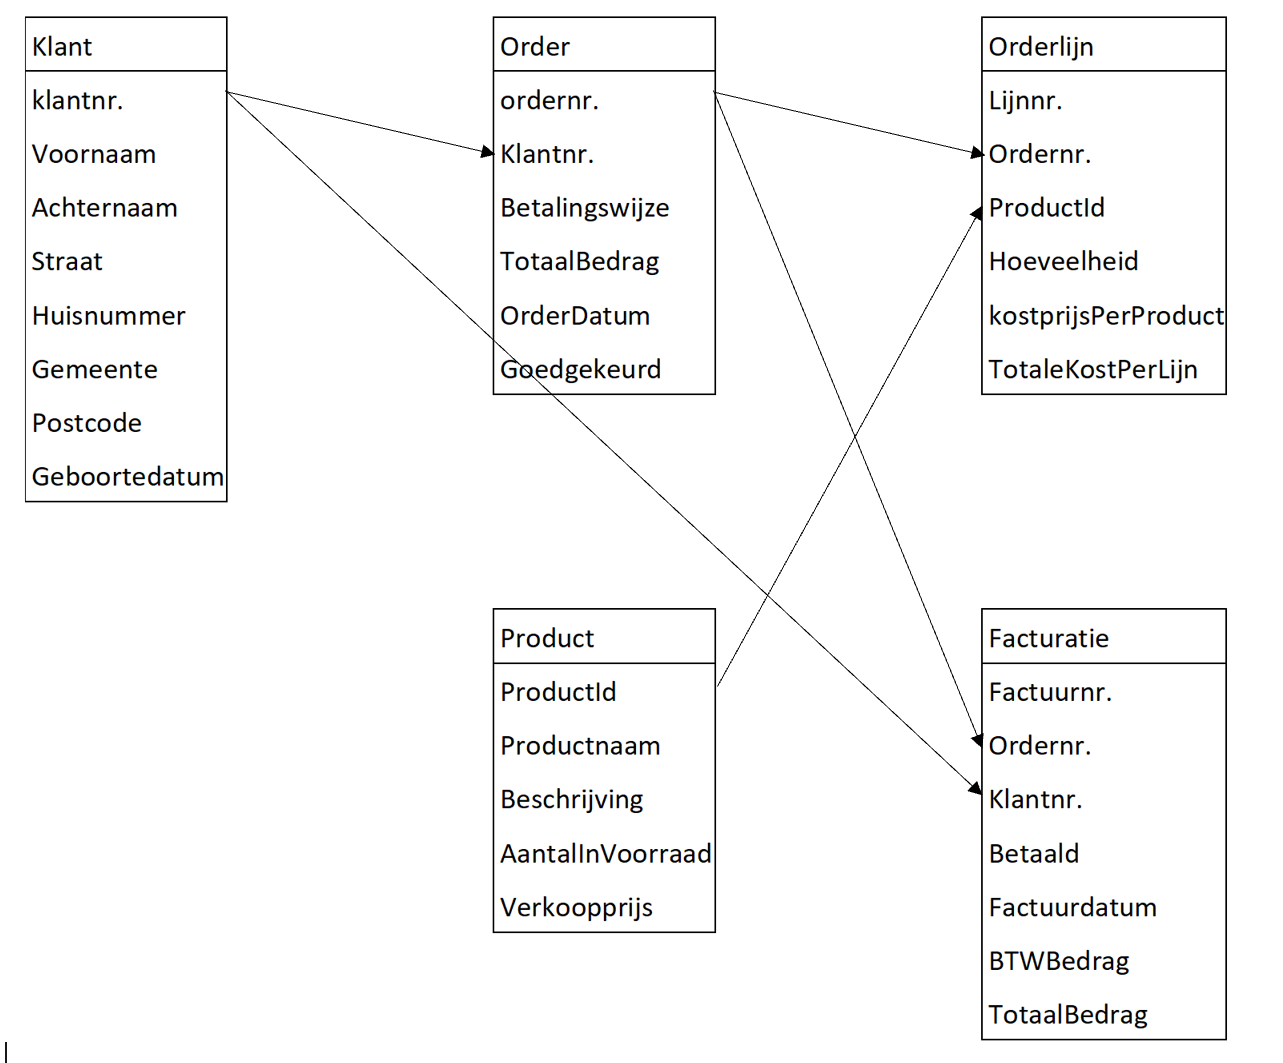
\includegraphics[width=15cm]{databank.png}
	\caption{De databank structuur.}
	\centering
\end{figure}

Een order weet wie zijn klant is. Credit management kan de eigenschap bij het order veranderen van 'goedgekeurd' naar 'niet goedgekeurd'. Van elk order wordt een orderlijn bijgehouden. Zodat er geweten is wat er op de order staat. Op elk orderlijn staat er een product of service. Van het product moet er een beschrijving en verkoopprijs zijn. Het aantal in voorraad is gekend omdat bij het order fullfilment moet de voorraad aangepast worden van het specifieke product. Een order en de klant zijn gekend op de facturatie. Zo kan er nagegaan worden of de factuur overeenkomt met wat er op het order staat. De klant zijn gegevens moeten gekend zijn om naar het juiste adres te factureren.

\section{De complete architectuur opbouwen}
Op figuur 3.3 is te zien hoe het proces in elkaar ziet. Door de microservice architectuur toe te passen op het order-to-cash proces verandert er niks aan de volgorde van het proces of het doel van het proces. De manier waarop gegevens worden opgehaald, verandert wel. 

\subsection{De communicatie tussen de onderdelen van het OTC proces}

\begin{figure}[h]
	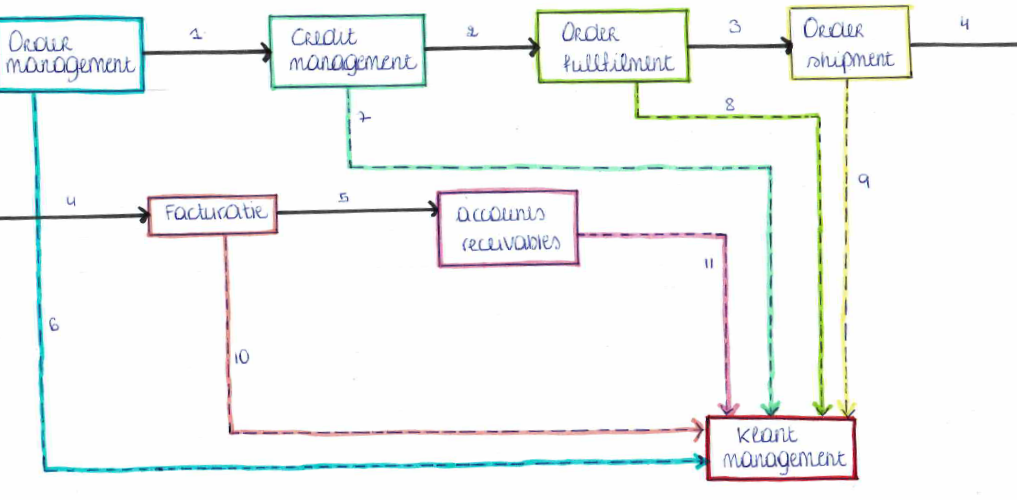
\includegraphics[width=15cm]{schema_communicatie.png}
	\caption{De communicatie tussen de verschillende onderdelen van het order-to-cash proces.}
	\centering
\end{figure}
Zoals al eerder vermeld, elk onderdeel van het OTC proces is een microservice. Elk onderdeel laat andere microservices het werk doen.
Op figuur 3.3 is het communicatie patroon zichtbaar.
Voordat het proces van start kan gaan, moet een klant een order plaatsen. Een order bevat een aantal producten. Eens de klant een order geplaatst heeft dan is er een ordernummer gekend. De klant staat bekend in het systeem met een klantnummer. Dat zijn twee belangrijke gegevens die veel gebruikt zullen worden.
Meer uitleg over wat elk onderdeel doet, bevindt zich in het volgende hoofdstuk.
De nummers van de opsomming komen overeen met die op afbeelding 3.2.
\begin{enumerate}
	\item De communicatie tussen ordermanagement en creditmanagement. Er is een order geplaatst door klant 66. Ordermanagement zorgt ervoor dat het order in de databank geraakt. Eens de taak van ordermanagement gedaan is, plaatst die het klantnummmer en het ordernummer op de queue van creditmanagement. Dan is zijn taak gedaan. Ordermanagement houdt zich niet bezig met wat er gebeurt nadat hij het bericht geplaatst heeft.
	\item De communicatie tussen creditmanagement en order fullfilment. Creditmanagement heeft het ordernummer en klantnummer van ordermanagement gekregen. Het bericht wordt van de queue gehaald. Creditmanagement gaat dan aan de hand van de klantgegevens beslissen of de klant het order mag plaatsen of niet. Is het order goedgekeurd dan wordt het ordernummer op de queue van order fullfilment gezet. Er moet niet worden teruggekeerd naar order management. Credit management heeft de rechten om het veld goedgekeurd aan te passen. De taak van creditmanagement is nu afgerond.
	\item De communicatie tussen order fullfilment en order shipment. Order fullfilment heeft het ordernummer doorgekregen van credit management. Order fullfilment geeft het ordernummer door aan order shipment eens zijn taak gedaan is. 
	\item De communicatie tussen order shipment en de facturatie. Het ordernummer werd op de queue van order shipment geplaatst. Eens alles opgemaakt is bij order shipment, wordt het ordernummer doorgestuurd naar de facturatie. De taak van order shipment is afgerond.
	\item De communicatie tussen facturatie en accounts receivables. De facturatie kreeg een bericht van order shipment om de factuur op te maken voor het order met des betreffende ordernummer. Is de taak van facturatie afgerond dan wordt de factuurnummer doorgestuurd naa accounts receivables. Zodat de betaling verder kan worden opgevolgd.
	\item Ordermanagement plaatst het ordernummer op de queue van klant management. Klant management stuurt een bevestiging naar de klant van het goed ontvangen van zijn/haar order. En laat weten dat er eerst een controle komt op het betaalbedrag van de klant.
	\item Creditmanagement plaatst het ordernummer en de status van goedgekeurd of afgekeurd op de queue. Dan wordt er een bericht verzonden naar de klant. Het bericht bevat de info of de klant zijn order is goedgekeurd of afgekeurd.
	\item Order fullfilment plaatst een bericht op de queue om te laten weten dat het order gemaakt is. Dat de goederen uit het magazijn zijn opgehaald en klaar gemaakt worden voor verzending.
	\item Order shipment plaatst een bericht op de queue wanneer de goederen klaar zijn voor vertrek. Klant management zorgt er dan voor dat het bericht tot bij de klant geraakt.
	\item Facturatie plaatst een bericht op de queue van klant management om ervoor te zorgen dat de factuur tot bij de klant geraakt.
	\item Accounts receivables plaatst een bericht op de queue van klant management als er aanmaningen moeten worden gestuurd.
\end{enumerate}

\subsection{De architectuur}
In volgende tabel, zijn er letters en bijhorende microservices terug te vinden. Deze worden gebruikt bij het uitleggen van de architectuur.
\begin{table}[]
	\resizebox{\textwidth}{!}{%
		\begin{tabular}{|l|p{15cm}|}
			\hline 
			A & Klantgegevens ophalen \\ \hline
			B & Orders plaatsen, ophalen en verwijderen \\ \hline
			C & Producten ophalen en het aantal van voorraad aanpassen \\ \hline
			D & Shipment documenten opstellen \\ \hline
			E & Facturatie maken en ophalen \\ \hline
			F & Aanmaning opmaken en verwijderen \\ \hline
			G & Bericht plaatsen op de queue \\ \hline
			H & Bericht ophalen van de queue \\ \hline
		\end{tabular}%
	}
	\caption{Legende die gebruikt wordt in de afbeeldingen.}
\end{table}

In tabel 3.2 is de legende terug te vinden die gebruikt wordt bij het uitleggen van elk onderdeel apart.
In figuur 3.3 is te zien hoe het volledige proces communiceert met de verschillende microservices. Elk onderdeel van het proces is een microservice op zich. Een microservice die meerdere microservices aanspreekt om goed te functioneren.
\begin{figure}[h]
	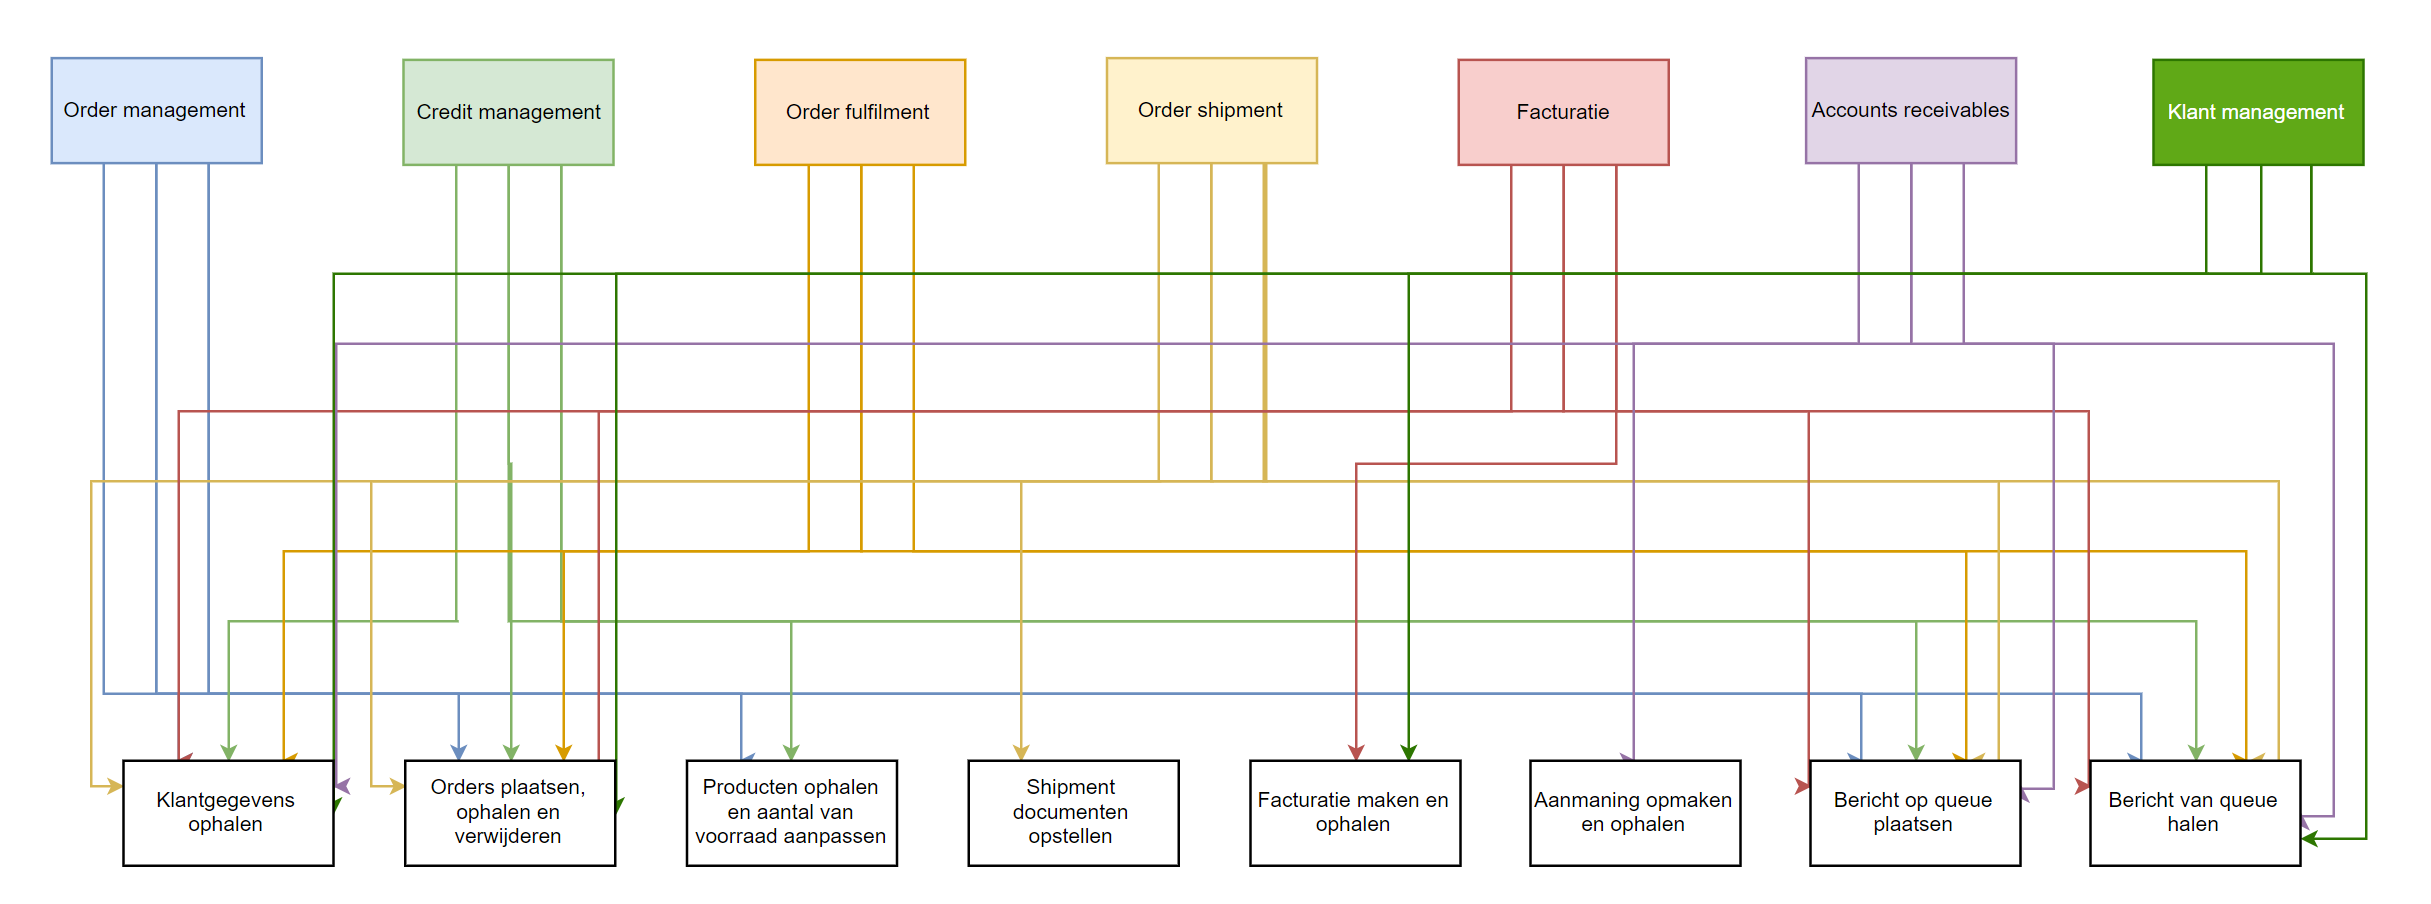
\includegraphics[width=15cm]{schema_microservices.png}
	\caption{Welk onderdeel, welke microservices aanspreekt.}
	\centering
\end{figure}

\subsubsection{Order management}
\begin{figure}[h]
	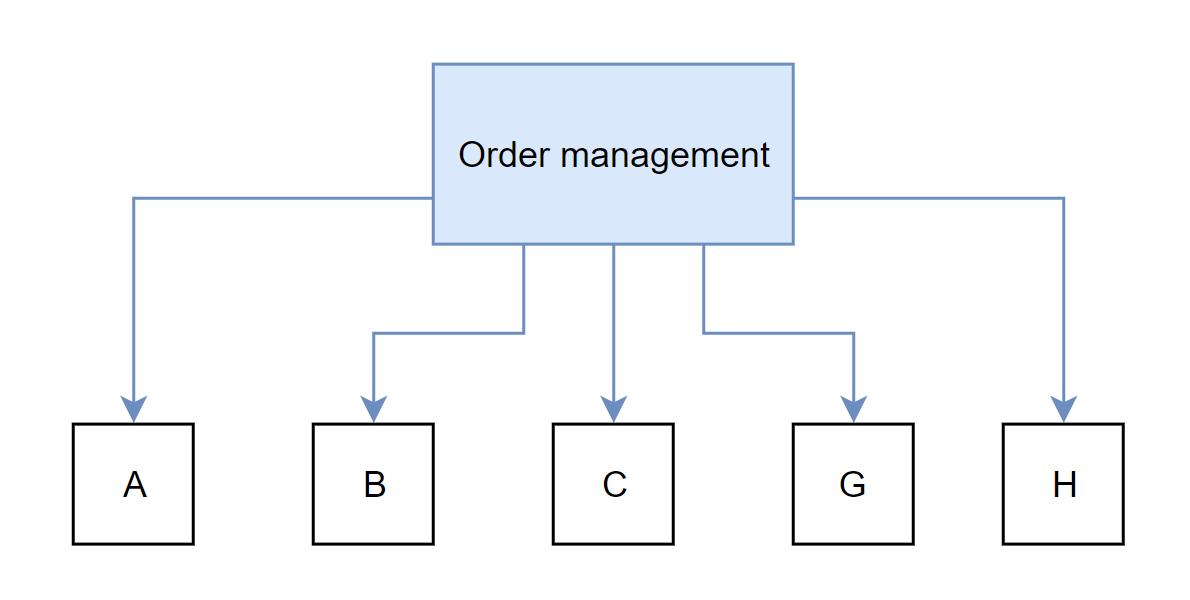
\includegraphics[width=5cm]{ordermanagement.png}
	\caption{Order management communiceert met volgende microservices.}
	\centering
\end{figure}
Order management communiceert met volgende microservices:
\begin{itemize}
	\item Klantgegevens ophalen.
	\item Orders plaatsen, ophalen en verwijderen.
	\item Producten ophalen en het aantal van de voorraad aanpassen.
	\item Bericht plaatsen op queue.
	\item Bericht van queue halen.
\end{itemize}
Een klant plaatst een order op het platform van het bedrijf. De gegevens van de klant worden opgehaald en gelinkt aan het nieuw gecreëerde order. Eens die twee taken zijn afgerond, wordt het bericht op de queue geplaatst van credit management.

\subsubsection{Credit management}
\begin{figure}[h]
	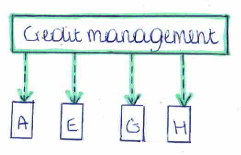
\includegraphics[width=5cm]{creditmanagement.png}
	\caption{Credit management communiceert met volgende microservices.}
	\centering
\end{figure}
Credit management communiceert met volgende microservices:
\begin{itemize}
	\item Klantgegevens ophalen.
	\item Orders ophalen, plaatsen en verwijderen.
	\item Facturatie maken en ophalen.
	\item Bericht plaatsen op queue.
	\item Bericht van queue halen.
\end{itemize}
Eerst wordt het bericht dat door order management op de queue geplaatst werd, opgehaald. Dan is er een klantnummer en een ordernummer. Bij credit management kijkt of de klant een goed betaalgedrag heeft. Staat de klant gekend als wanbetaler dan naar het order gegaan om de plaatsing van het order af te keuren. In andere gevallen krijgt de order een goedkeuring en wordt het ordernummer geplaatst op de queue van order fullfilment. Dan zit de taak van credit management erop.

\subsubsection{Order fullfilment}
\begin{figure}[h]
	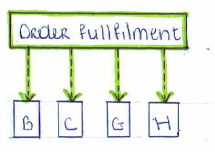
\includegraphics[width=5cm]{orderfullfilment.png}
	\caption{Order fullfilment communiceert met volgende microservices.}
	\centering
\end{figure}
Order fullfilment communiceert met volgende microservices:
\begin{itemize}
	\item Orders ophalen, plaatsen en verwijderen.
	\item Producten ophalen en het aantal in de voorraad aanpassen.
	\item Bericht plaatsen op queue.
	\item Bericht van queue halen.
\end{itemize}
Bij order fullfilment staat er een ordernummer op de queue. Die wordt opgehaald en aan de hand van het ordernummer, weet men welke goederen er uit het magazijn moeten gehaald worden. Voor alle goederen moet het aantal in de voorraad aangepast worden. Eens het order compleet is, wordt het ordernummer op de queue van order shipment geplaatst.

\subsubsection{Order shipment}
\begin{figure}[h]
	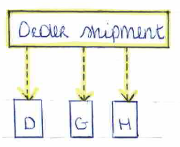
\includegraphics[width=5cm]{ordershipment.png}
	\caption{Order shipment communiceert met volgende microservices.}
	\centering
\end{figure}
Order shipment communiceert met volgende microservices:
\begin{itemize}
	\item Orders ophalen, plaatsen en verwijderen.
	\item Klantgegevens ophalen.
	\item Shipment document opstellen.
	\item Bericht plaatsen op queue.
	\item Bericht van queue halen.
\end{itemize}
Order shipment krijgt het ordernummer binnen via zijn queue. Het order wordt bekeken en de klant gegevens worden opgehaald aan de hand van het gekoppelde klantnummer aan het order. Eens het order shipment document is opgesteld en alle goederen klaar zijn voor vertrek, wordt het ordernummer geplaatst op de queue van facturatie.

\subsubsection{Facturatie}
\begin{figure}[h]
	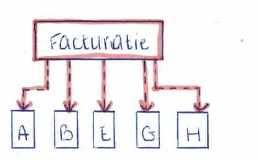
\includegraphics[width=5cm]{facturatie.png}
	\caption{Facturatie communiceert met volgende microservices.}
	\centering
\end{figure}
Facturatie communiceert met volgende microservices:
\begin{itemize}
	\item Klantgegevens ophalen.
	\item Orders ophalen, plaatsen en verwijderen.
	\item Facturatie maken en ophalen.
	\item Bericht plaatsen op queue.
	\item Bericht van queue halen.
\end{itemize}
Eens het ordernummer opgehaald is van de queue, wordt alle nodig info opgehaald om de factuur op te maken. De nodige gegevens zijn klantgegevens en het order. Eens de factuur opgemaakt is, wordt het factuur nummer geplaatst op de queue van account receivables.

\subsubsection{Accounts receivables}
\begin{figure}[h]
	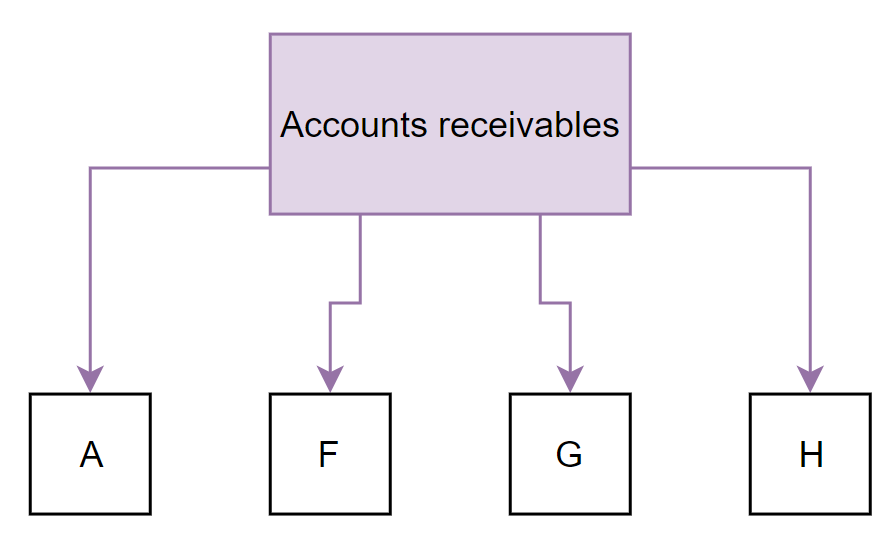
\includegraphics[width=5cm]{accountreceivables.png}
	\caption{Accounts receivables communiceert met volgende microservices.}
	\centering
\end{figure}
Accounts receivable gaat na of de betaling wel goed wordt afgerond. Om dit te kunnen, worden volgende microservices aangesproken:
\begin{itemize}
	\item Klantgegevens ophalen.
	\item Facturatie maken en ophalen.
	\item Bericht plaatsen op queue.
	\item Bericht van queue halen.
\end{itemize}

\subsubsection{Klant management}
\begin{figure}[h]
	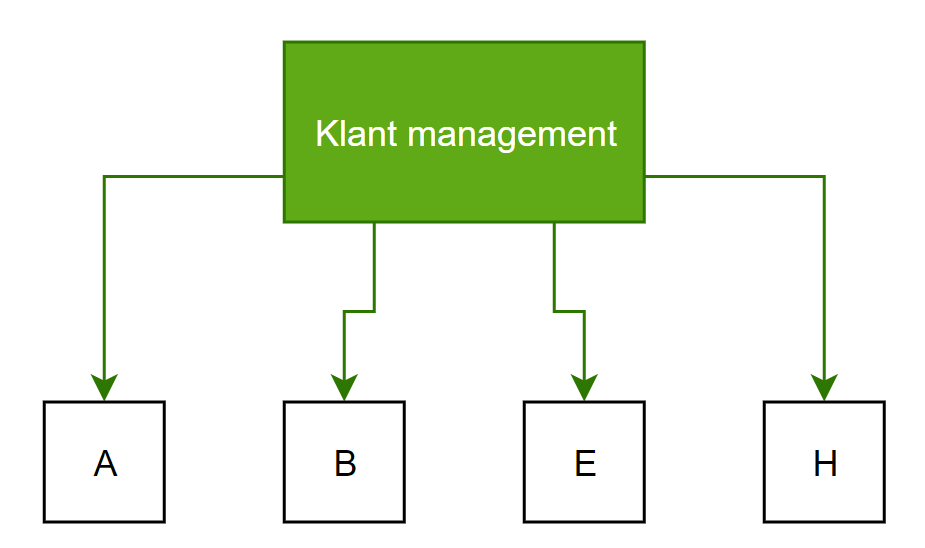
\includegraphics[width=5cm]{klantmanagement.png}
	\caption{Klant management communiceert met volgende microservices.}
	\centering
\end{figure}
Klant management staat in voor het contact met de klant. Dit deel gebruikt volgende microservices:
\begin{itemize}
	\item Klantgegevens ophalen.
	\item Orders ophalen, plaatsen en verwijderen.
	\item Facturatie maken en ophalen.
	\item Bericht van queue halen.
\end{itemize}
Als een van de vorige onderdelen een bericht plaatst op de queue, zal die verwerkt worden en de nodige info wordt opgehaald.

\subsection{De volgende stappen: Het toevoegen van API, logging en authenticatie en authorisatie}
\subsubsection{Logging}
Logging kan toegepast worden door nog een extra microservice te ontwikkelen. Hiernaar kunnen de andere microservices hun logs posten. Hier zal niet verder op worden ingegaan. 

\subsubsection{API gateway}
Een API gateway wordt toegevoegd om ervoor te zorgen dat de architctuur niet openbaar is voor iedereen. Er is één aanspreekpunt en die regelt de rest van de communicatie.
De API communiceert in dit geval enkel met order management. De API geeft alle nodige informatie door en order management schrijft deze weg naar de datastore en naar de databank.
\begin{figure}[h]
	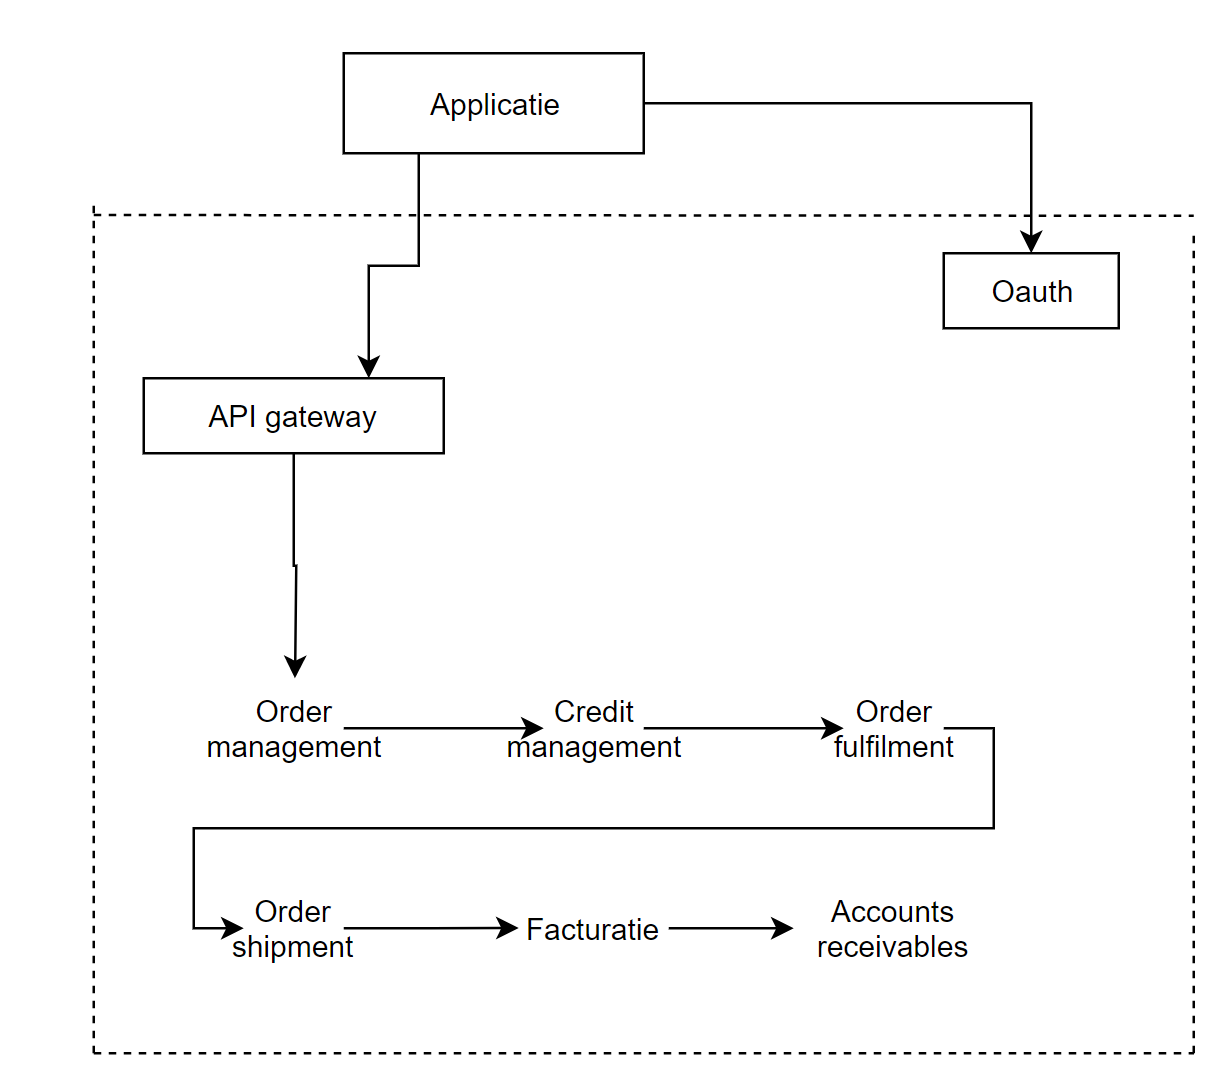
\includegraphics[width=10cm]{apiSchema.png}
	\caption{Vereenvoudigd schema.}
	\centering
\end{figure}

\subsubsection{Authenticatie en autorisatie}
Onder het hoofdstuk 'stand van zaken', is een vergelijking te vinden over authenticatie. Uit die vergelijking, is de keuzen API gekozen als authenticatie. Binnen API zijn er verschillende opties, die worden ook overlopen in het vorige hoofdstuk. Er is gekozen voor OAuth omdat dit de meest bekende en gebruikte versie is.

De gebruiker moet gekend zijn voordat die een order kan plaatsen. De authenticatie van de gebruiker gebeurt vooraf. Er is een aparte micrservice voor authenticatie. Hier wordt niet dieper op in gegaan.
Op afbeelding 3.12 is wel een mogelijke plaatsing zichtbaar.


